\section{Queue 队列}

Queue 继承自 Collection 接口,表示单端队列,遵循 FIFO(先进先出) 规则。Deque 继承自 Queue,表示双端队列,两端都可以插删元素:

\begin{Java}
public interface Queue<E> extends Collection<E>
public interface Deque<E> extends Queue<E>
\end{Java}

这两个接口定义的方法比较少,根据 因为容量问题而导致操作失败后处理方式的不同 可以分为两类方法: 一种在操作失败后会抛出异常,另一种则会返回特殊值。

\begin{table}[H]
    \centering
    \small
    \caption{队列接口}
    \label{table:队列接口}
    \setlength{\tabcolsep}{4mm}
    \begin{tabular}{c|c|cc}
        \toprule
        \textbf{接口} & \textbf{方法} & \textbf{抛异常} & \textbf{返回值} \\
        \midrule
        \multirow{3}{*}{\textbf{Queue}} & 插入队尾 & add(E e) & offer(E e) \\
        & 删除队首 & remove() & poll() \\
        & 查询队首元素 & element() & peek() \\
        \midrule
        \multirow{6}{*}{\textbf{Deque}} & 插入队首 & addFirst(E e) & offerFirst(E e) \\
        & 插入队尾 & addLast(E e) & offerLast(E e) \\
        & 删除队首 & removeFirst() & pollFirst() \\
        & 删除队尾 & removeLast() & pollLast() \\
        & 查询队首元素 & getFirst() & peekFirst() \\
        & 查询队尾元素 & getLast() & peekLast() \\
        \bottomrule
    \end{tabular}
\end{table}

Deque 还有 push 和 pop 方法,模拟栈操作。

\begin{center}
    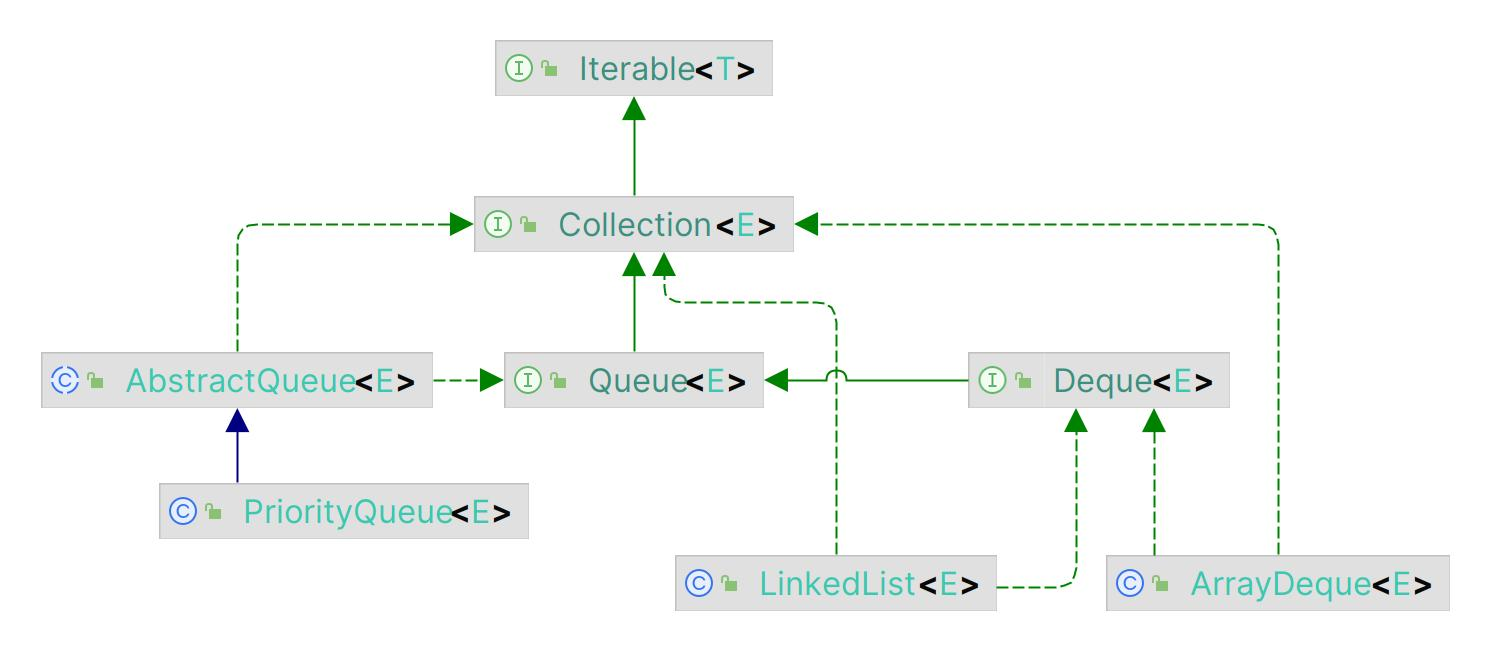
\includegraphics[width=0.7\linewidth]{../../imgs/Queue.jpg}
\end{center}

Queue 有一个抽象类 AbstractQueue,看一下它的方法实现就知道,抛异常和返回值函数之间的关系了。

\begin{Java}
public boolean add(E e) {
    if (offer(e))
        return true;
    else
        throw new IllegalStateException("Queue full");
}
\end{Java}

可以发现,抛异常函数本质是对返回值函数的进一步封装。

\subsection{PriorityQueue}

PriorityQueue 是优先队列,优先队列的作用是能保证每次取出的元素都是队列中权值最小的(默认为元素本身的自然顺序)。

\begin{Java}
public class PriorityQueue<E> extends AbstractQueue<E> implements java.io.Serializable
\end{Java}

在底层,PriorityQueue 使用数组+小根堆\footnote{参考文章:\url{https://blog.csdn.net/Zj_boring/article/details/105157360}}存储数据。小根堆的实现还是比较简单的,建议读者先了解一下。

\begin{Java}
transient Object[] queue;
public PriorityQueue() {
    this(DEFAULT_INITIAL_CAPACITY, null);
}
\end{Java}

让我们看一下常规操作的实现,增加元素,小根堆增加元素默认增加在队尾:

\begin{Java}
public boolean add(E e) {
    return offer(e);
}

public boolean offer(E e) {
    if (e == null)
        throw new NullPointerException();
    modCount++;
    int i = size;
    if (i >= queue.length)
        grow(i + 1);
    siftUp(i, e);
    size = i + 1;
    return true;
}
\end{Java}

我们发现,add 和 offer 没有严格按照抛异常和返回值区分开来,其他几个方法也类似。

这里有两个重要的方法,shiftUp 是元素插入数组尾部,小根堆自底向上递归重构的函数,涉及具体算法,不讲。grow 是数组扩容,注释写的非常明了:容量小于 64,扩容到两倍,否则扩容到 1.5 倍。

\begin{Java}
private void grow(int minCapacity) {
    int oldCapacity = queue.length;
    // Double size if small; else grow by 50%
    int newCapacity = ArraysSupport.newLength(oldCapacity,
            minCapacity - oldCapacity, /* minimum growth */
            oldCapacity < 64 ? oldCapacity + 2 : oldCapacity >> 1
                                       /* preferred growth */);
    queue = Arrays.copyOf(queue, newCapacity);
}
\end{Java}

其余几个操作如下:
\begin{itemize}
    \item boolean remove(Object o): 删除指定元素,没用无参数的函数重载。
    \item E poll(): 删除队首元素并返回。
    \item E peek(): return (E) queue[0];
    \item E element(): 调用 peek,没有则抛错。
\end{itemize}

\subsection{ArrayDeque}

ArrayDeque 顾名思义,是使用数组实现的双向队列,是 Queue 的首选实现(其次是 LinkedList),同时也是栈结构的首选实现(Java 不推荐使用 Stack)。

\begin{Java}
public class ArrayDeque<E> extends AbstractCollection<E> implements Deque<E>, Cloneable, Serializable
\end{Java}

ArrayDeque 底层采用数组存储数据,同时维护两个指向头部和尾部元素的引用:

\begin{Java}
transient Object[] elements;
transient int head;
transient int tail;
\end{Java}

如何判断头部和尾部引用呢,头部前一个元素为空,尾部后一个元素为空。因此必须有一个空元素,默认构造函数就预留了一单位的空间:

\begin{Java}
public ArrayDeque() {
    elements = new Object[16 + 1];
}
\end{Java}

\begin{figure}[H]
    \centering
    \begin{tikzpicture}[scale = 1]
        \matrix [nodes = {minimum height=10mm, text width=1cm, align=center, color = black!50}] at (0,-0.78)
        {
            \node {0}; & \node {1}; & \node {2}; & \node {3} ; & \node {4}; & \node {5}; & \node {6}; & \node {7};\\
        };
        \matrix [nodes = {draw, fill=black!5, minimum height=10mm, text width=1cm, align=center}] at (0,0)
        {
            \node (0) {}; & \node (1) {6}; & \node (2) {5}; & \node(3) {3} ; & \node(4) {8}; & \node(5) {7}; & \node(6) {}; & \node(7) {};\\
        };
        \node[font=\small] (head) at (-3,1.5) {head};
        \node[font=\small] (tail) at (2,1.5) {tail};
        \draw[-Stealth] (head) -- (1);
        \draw[-Stealth] (tail) -- (5);
     \end{tikzpicture}
    \caption{ArrayDeque 内部结构}
    \label{fig:ArrayDeque 内部结构}
\end{figure}

删除和查找操作没什么好说的,唯一注意的是指针可能会在头部和尾部之间跳转,在插入操作中一并说明,看一下增加操作。

\begin{Java}
public void addFirst(E e) {
    if (e == null)
        throw new NullPointerException();
    final Object[] es = elements;
    es[head = dec(head, es.length)] = e;
    if (head == tail)
        grow(1);
}

static final int dec(int i, int modulus) {
    if (--i < 0) i = modulus - 1;
    return i;
}
\end{Java}

扩容操作就不说了,小则两倍,大则增加 50\%。这里有个 dec 函数,是为了防止头部指向下标为 0 的区域,如果不是,则直接在 head-1 位置插入元素,否则,在尾部插入元素。

其他就没什么好讲的了,扩容是通过 native 的 copyOf 方法。

\newpage